Under the condition of \textbeta-stable, the proton's contribution $x_p = \rho_p/\rho_b$ to the baryon density of of \gls{NM} is given by Figure \ref{fig:xp}
\begin{figure}[ht!]
        \centering
        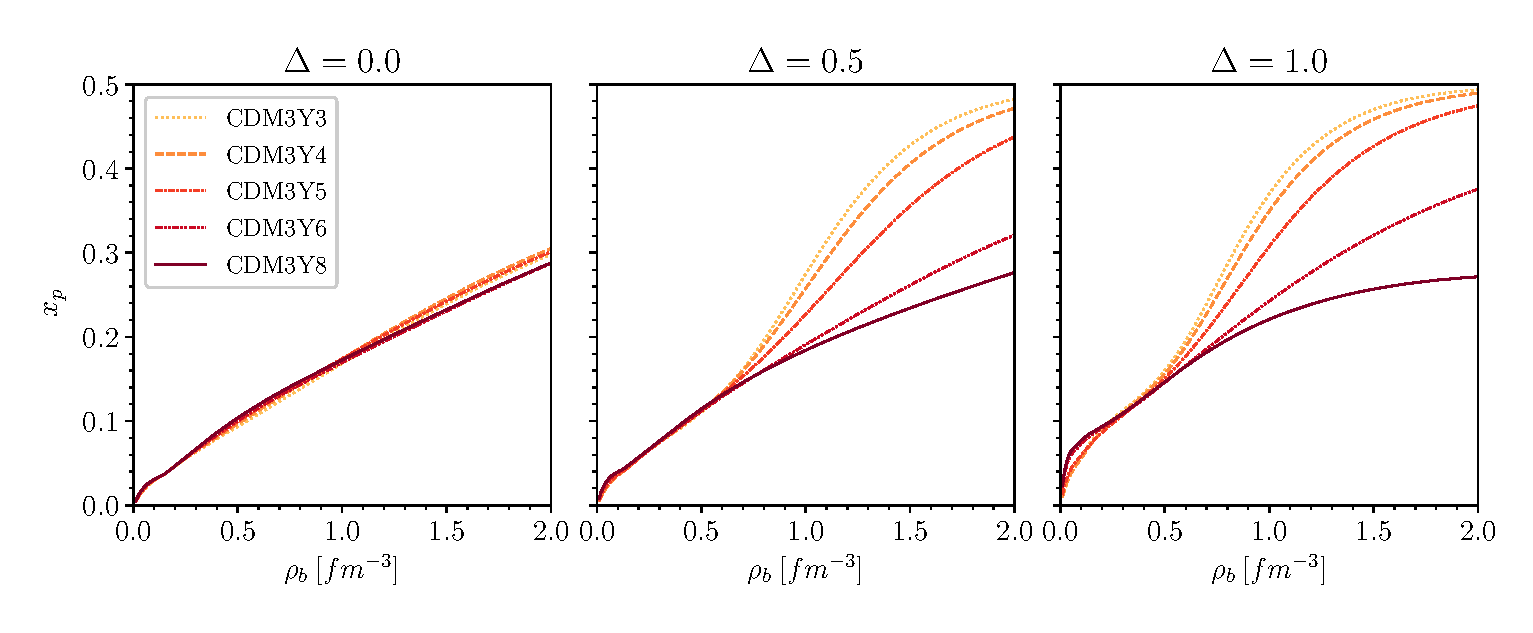
\includegraphics[width=\textwidth]{fig/xp.eps}
        \caption{Proton fraction $x_p$ of \textbeta-stable \gls{NM} at different baryon density and spin polarity for CDM3Y$n$ interactions. The lower horizontal lines are the \gls{DU} threshold. The dot at the end of each line corresponds to the highest mass \gls{NS}'s central density of each model.}
        \label{fig:xp}
\end{figure} 
\begin{figure}[ht!]
        \centering
        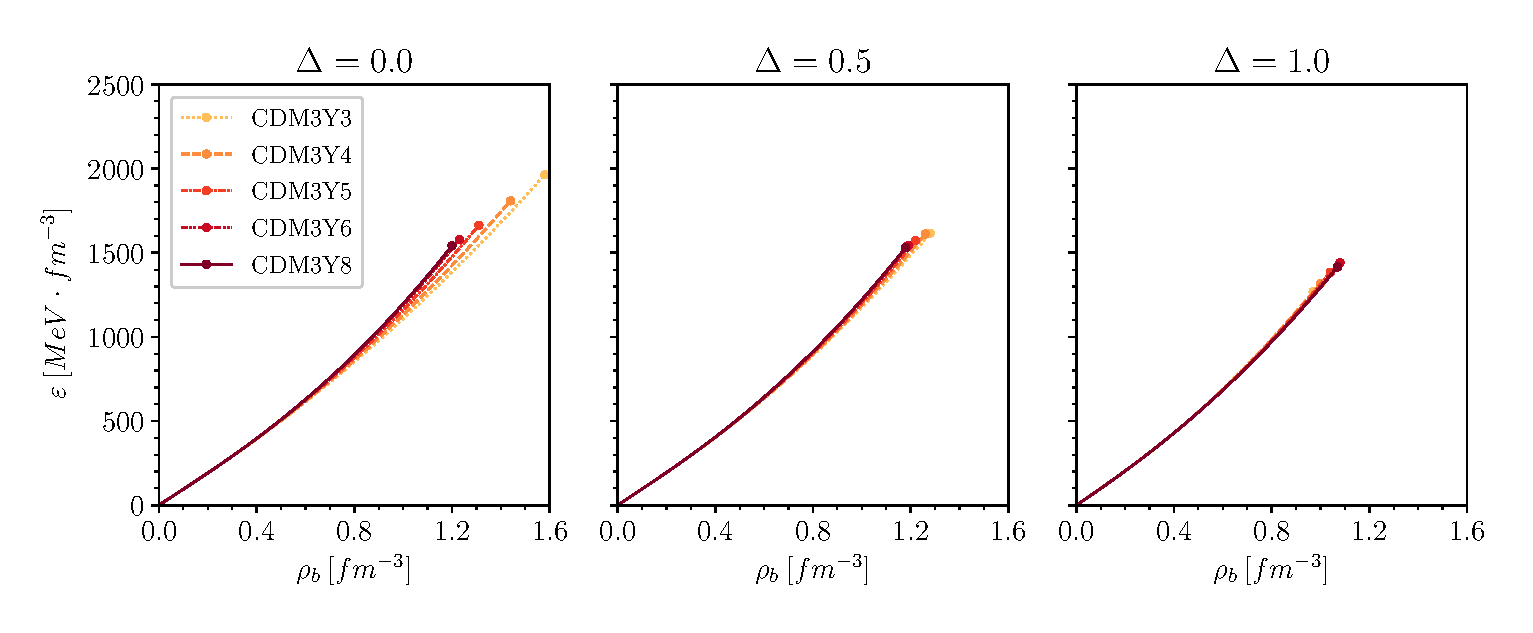
\includegraphics[width=\textwidth]{fig/E.eps}
        \caption{Total mass-energy density $\varepsilon$ of \textbeta-stable \gls{NM} at increasing spin polarity with 6 CDM3Y$n$ interaction models. The dot at the end of each line corresponds to the highest mass \gls{NS}'s central density of each model.}
        \label{fig:e}
\end{figure} 
\begin{figure}[ht!]
        \centering
        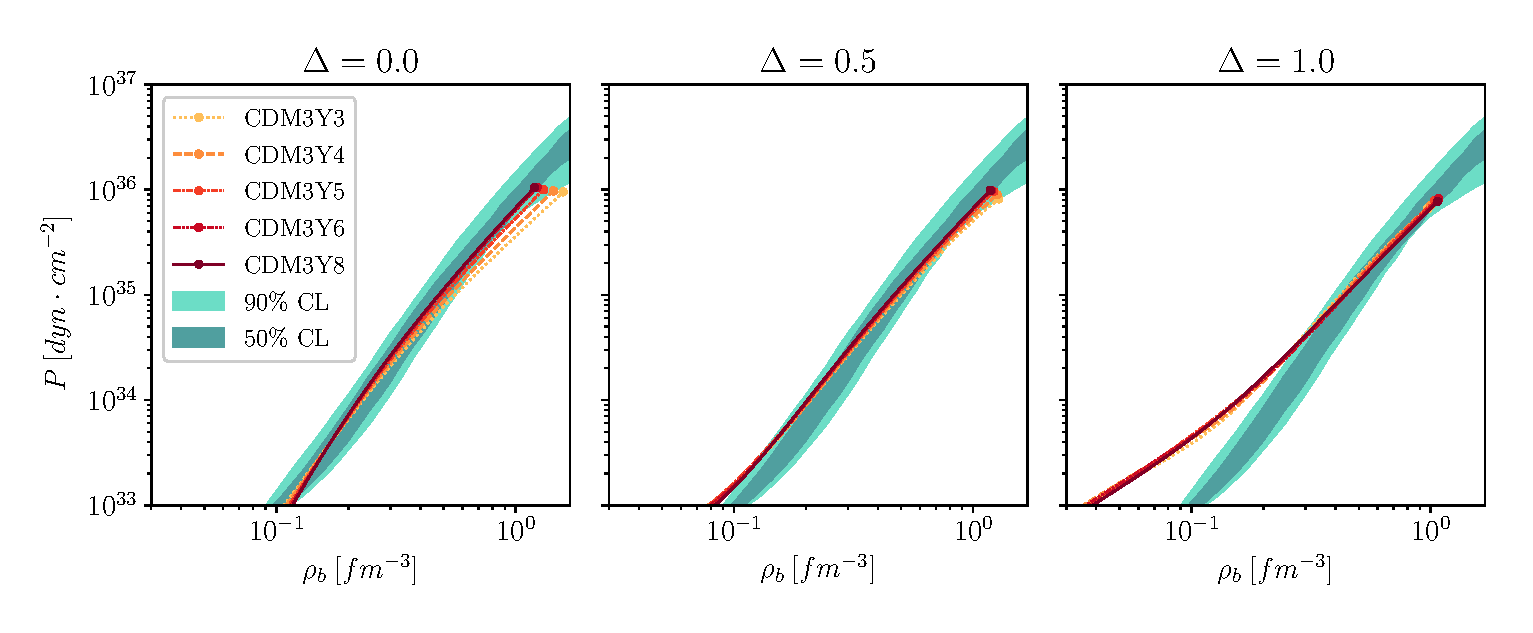
\includegraphics[width=\textwidth]{fig/P.eps}
        \caption{Same as Figure \ref{fig:e} for the pressure $P$ along with empirical pressure given by the ``Spectral'' \gls{EoS} from the Bayesian analysis of the GW170817 data \citep{abbott2018gw170817} with 50\% (light gray) and 90\% (dark gray) confidence level. The dot at the end of each line corresponds to the central baryon density $\rho_b$ of maximum \gls{NS} mass.}
        \label{fig:p}
\end{figure} 
\begin{figure}[ht!]
        \centering
        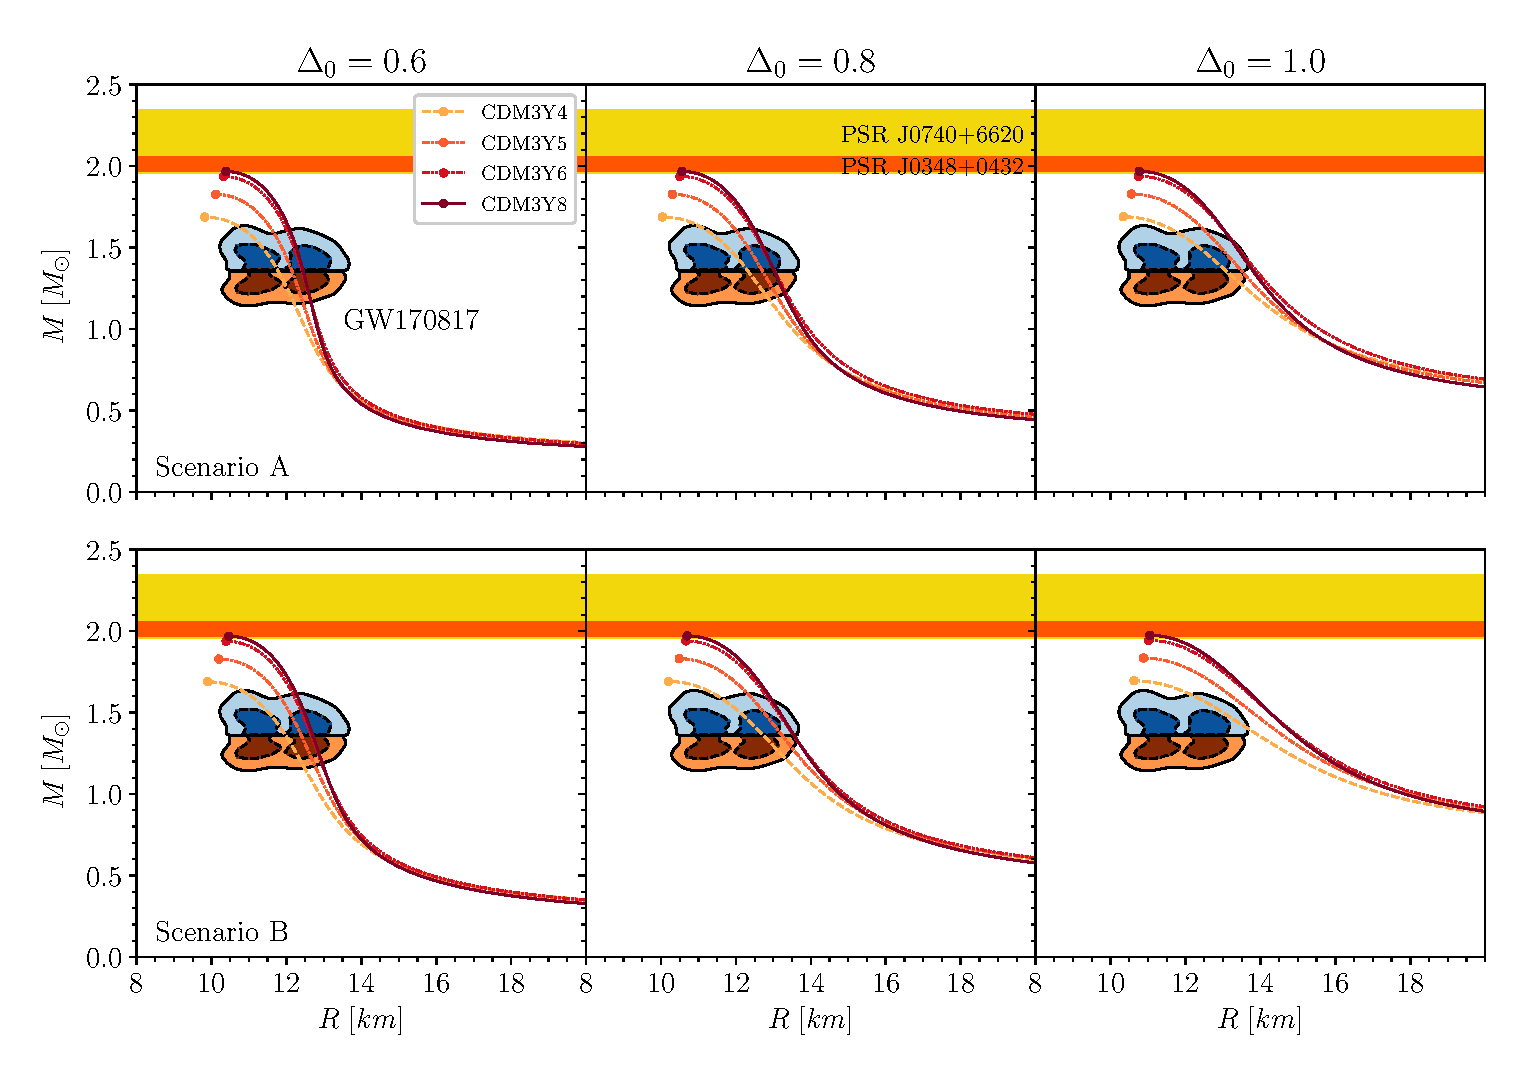
\includegraphics[width=\textwidth]{fig/MR.eps}
        \caption{The relation between gravitational mass $M$ and the radius $R$ of the \gls{NS} according to the corresponding model and polarity. The GW170817 constraint for \gls{NS} with mass $1.4M_\odot$ is shown by the colored contour, where the blue (red) shaded area represents the heavier (lighter) \gls{NS} \citep{abbott2018gw170817}. The dot in each line indicates the maximum \gls{NS} mass of the each model.}
        \label{fig:mr}
\end{figure} 
\begin{figure}[ht!]
        \centering
        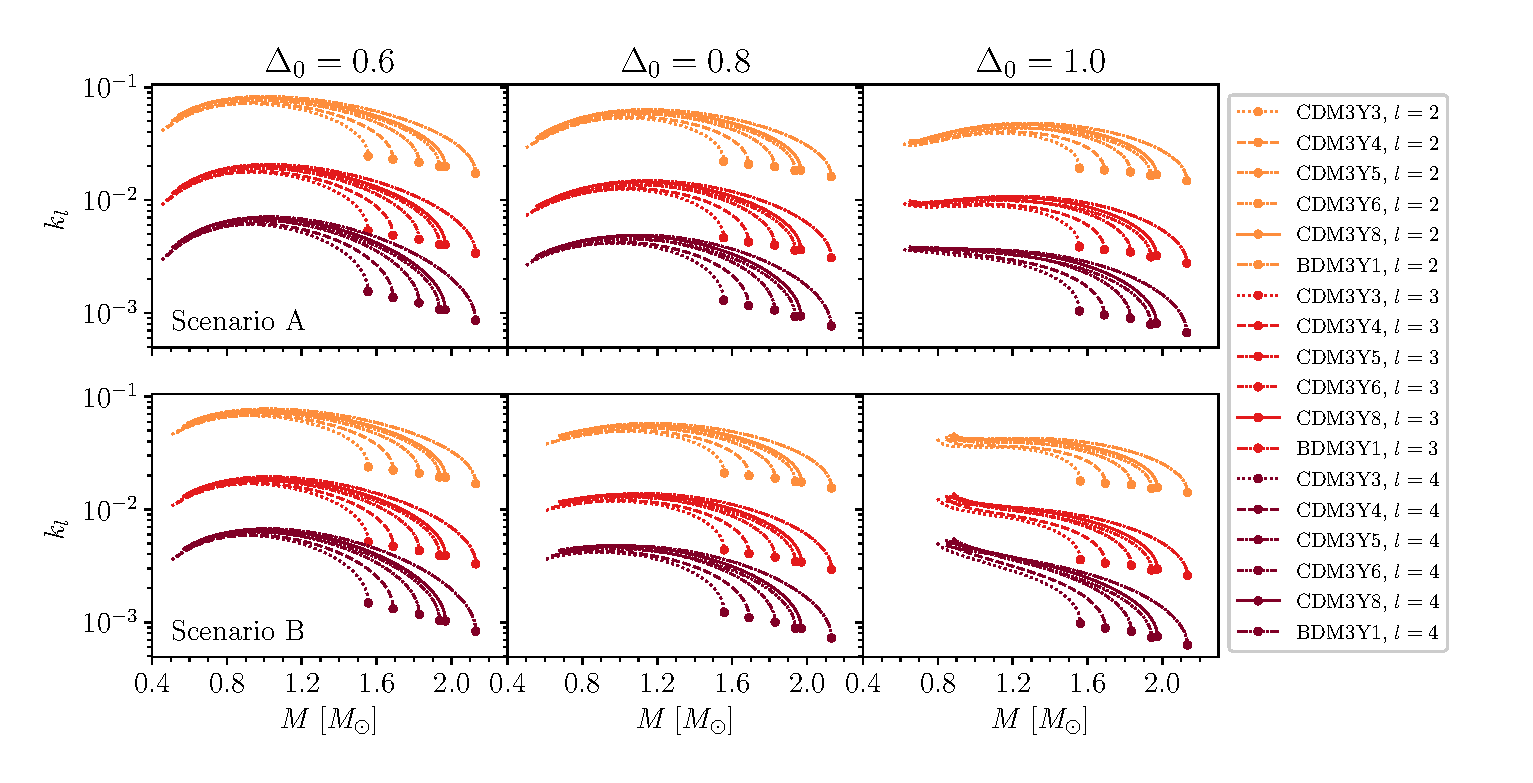
\includegraphics[width=\textwidth]{fig/kl.eps}
        \caption{\gls{GE} tidal Love number at $l$\textsuperscript{th} order $k_l$ as function of \gls{NS} mass computed with CDM3Y$n$ models at different spin polarities.}
        \label{fig:kl}
\end{figure} 
\begin{figure}[ht!]
    \centering
    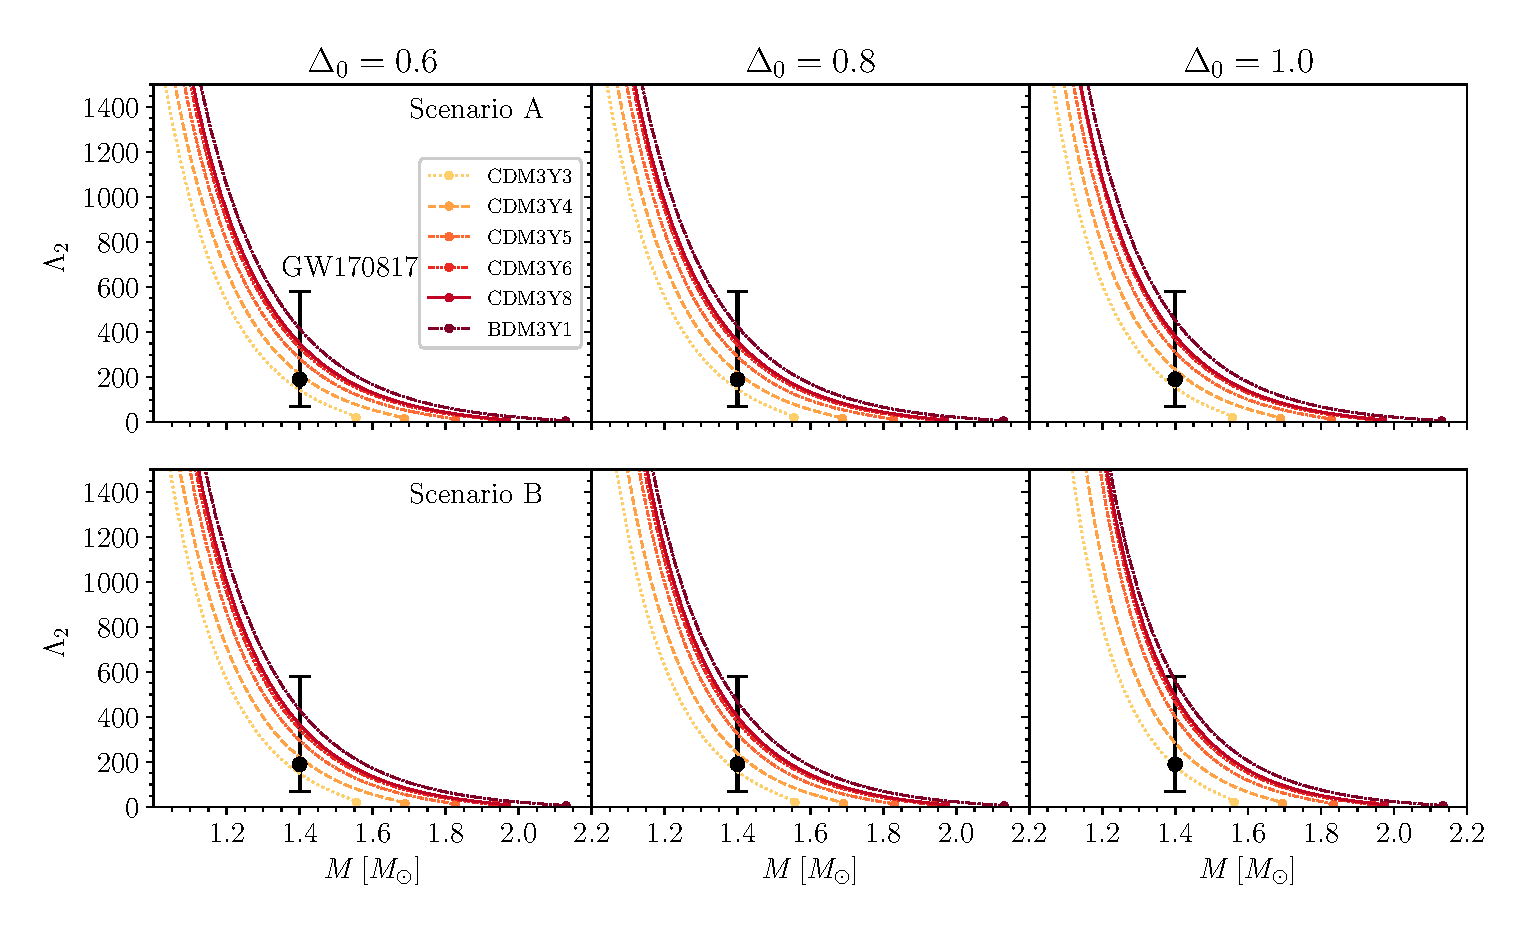
\includegraphics[width=\textwidth]{fig/Lambda2.eps}
    \caption{Dimensionless \gls{GE} tidal deformability parameter of 2\textsuperscript{nd} order $\Lambda_2$ of different CDM3Y$n$ models with varying $\Delta$. The vertical bar is the empirical tidal deformability constraint at $1.4M_\odot$, obtained from the Bayesian analysis of GW170817 data at 90\% confidence level \cite{abbott2018gw170817}.}
    \label{fig:Lambda2}
\end{figure} 
\begin{figure}[ht!]
        \centering
        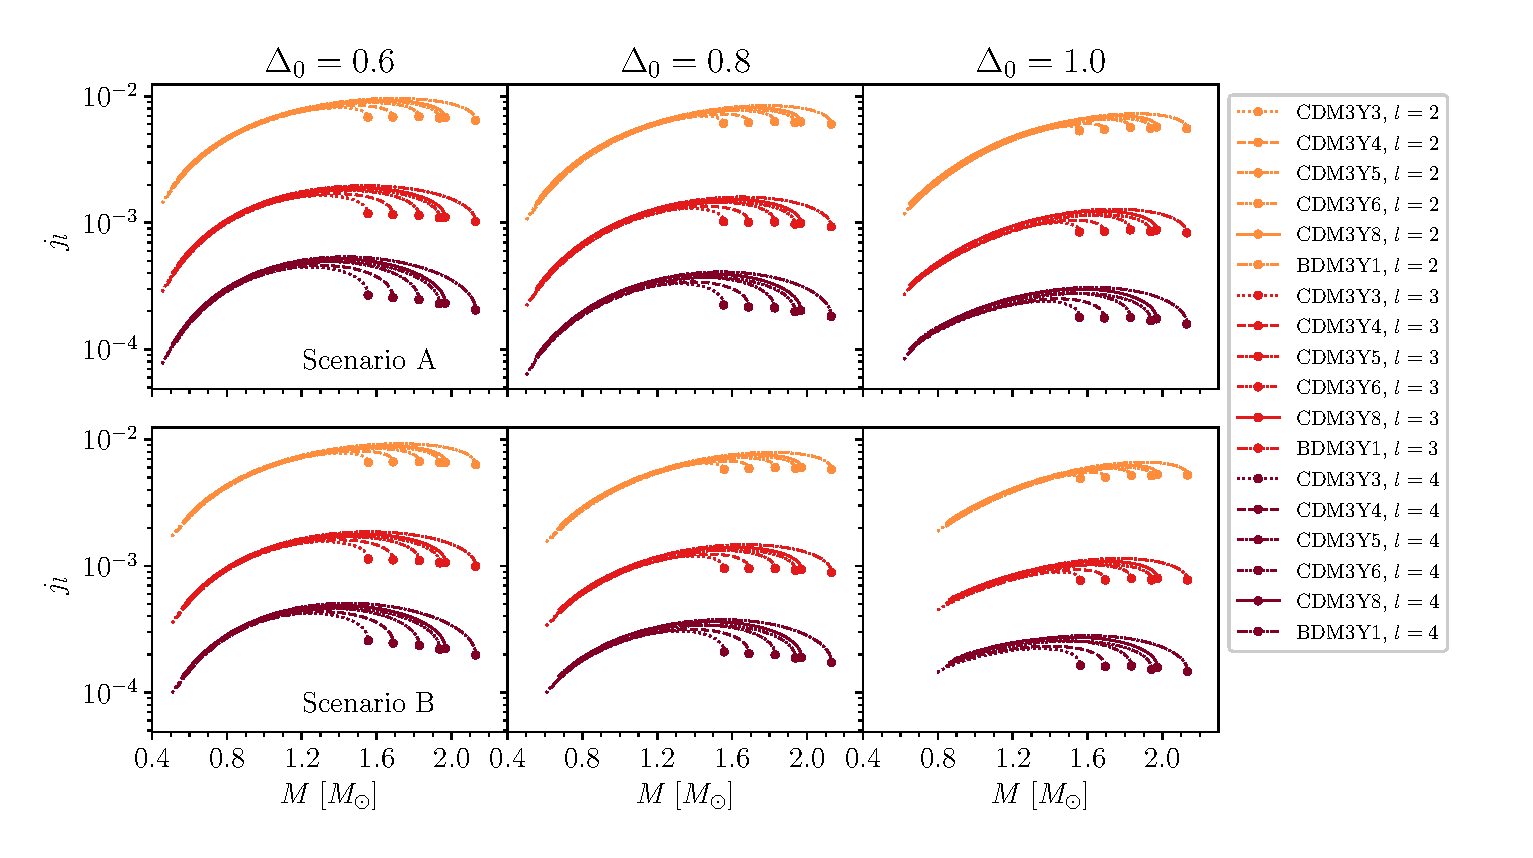
\includegraphics[width=\textwidth]{fig/jl_stat.eps}
        \caption{\gls{GM} tidal Love number at $l$\textsuperscript{nd} order $j_l$ as function of \gls{NS} mass computed with CDM3Y$n$ models of \emph{strictly static fluid} at different polarities.}
        \label{fig:jl_stat}
\end{figure} 
\begin{figure}[ht!]
        \centering
        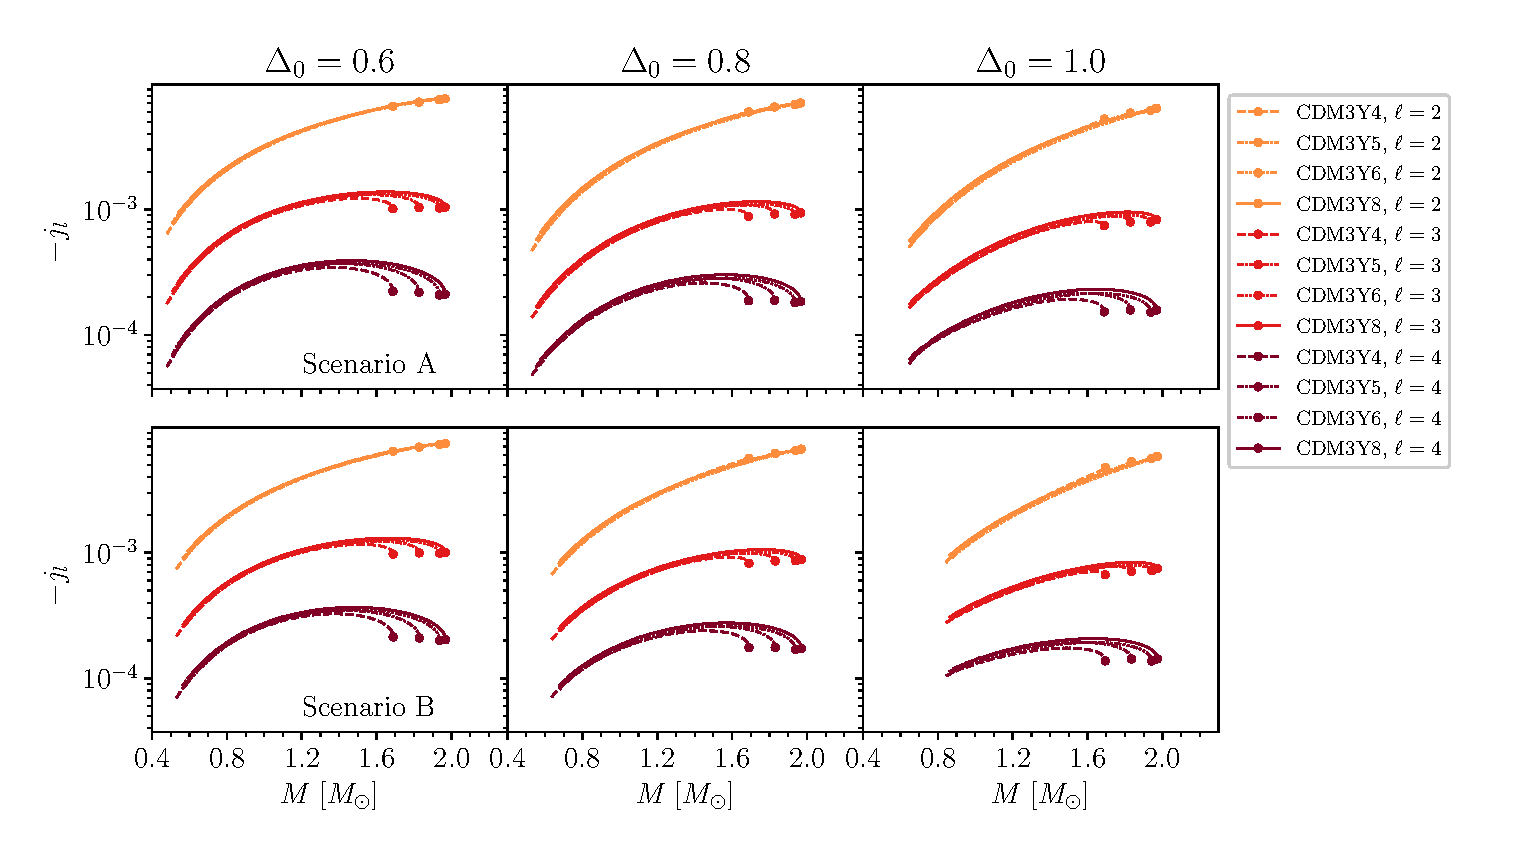
\includegraphics[width=\textwidth]{fig/jl_irrot.eps}
        \caption{\gls{GM} tidal Love number at $l$\textsuperscript{nd} order $j_l$ as function of \gls{NS} mass computed with CDM3Y$n$ models of \emph{irrotational fluid} at different polarities.}
        \label{fig:jl_irrot}
\end{figure} 
